\begin{myConceptSteps}{To find the slope of a line from its graph\dots}
    \myStep{plot}{Plot any two points that are on the line}
    \myStep{find}{
        Find the coordinates of both point. 
        Let's call them $(x_1,y_1)$ and $(x_2,y_2)$.
        (Which point is $1$ and which is $2$ does not matter.)
    }
    \myStep{calculate}{
        Calculate the slope as the \emph{rise over run}: 
        $m = (y_2-y_1) / (x_2 - x_1)$.
    }
\end{myConceptSteps}


\myBlankExample{1.5in}{
    Find the slope of this line.
    \begin{center}
        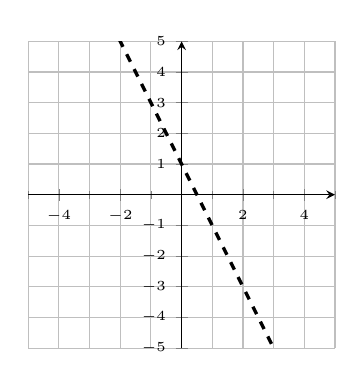
\begin{tikzpicture}
            \begin{axis}[
                width=2.5in,
                grid=both,
                axis x line = middle,axis y line = middle,
                axis equal image,
                xtick distance = 2, ytick distance = 1, 
                minor x tick num = 1,
                xmin = -5, xmax=5,
                ymin = -5, ymax=5,
                tick label style = {font=\tiny},
                ]
                \addplot[dashed,style={line width=1.2pt},no marks, samples=3, domain=-3:4, ] expression { -2*x + 1 };
            \end{axis}
        \end{tikzpicture}
    \end{center}
}


\myBlankExample{1.25in}{
    Find the slope of this line.
    \begin{center}
        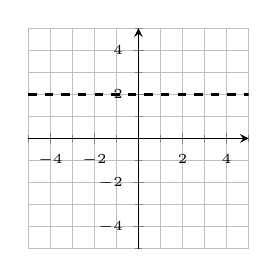
\begin{tikzpicture}
            \begin{axis}[
                width=2.in,
                grid=both,
                axis x line = middle,axis y line = middle,
                axis equal image,
                xtick distance = 2, ytick distance = 2, 
                minor tick num = 1,
                xmin = -5, xmax=5,
                ymin = -5, ymax=5,
                tick label style = {font=\tiny},
                ]
                \addplot[dashed,style={line width=1.2pt}, no marks, samples=3, domain=-5:5, ] expression { 2 };
            \end{axis}
        \end{tikzpicture}
    \end{center}
}

\myBlankExample{2in}{
    Find the slope of this line.
    \begin{center}
        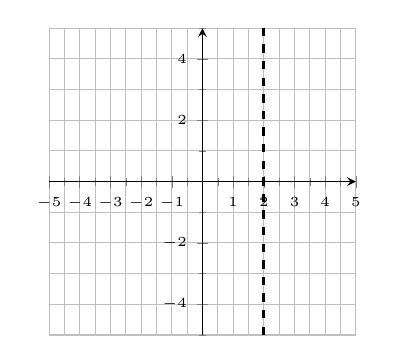
\begin{tikzpicture}
            \begin{axis}[
                width=2.5in,
                grid=both,
                axis x line = middle,axis y line = middle,
                axis equal image,
                xtick distance = 1, ytick distance = 2, 
                minor tick num = 1,
                xmin = -5, xmax=5,
                ymin = -5, ymax=5,
                tick label style = {font=\tiny},
                ]
                \addplot +[mark=none,dashed,style={line width=1.2pt}, black] coordinates {(2, -5) (2, 5)};
            \end{axis}
        \end{tikzpicture}
    \end{center}
}